\chapter{Введение}

\section{Цель работы}

Изучить параметры виброакустического канала утечки информации.

Для выполнения работы используется модель канала утечки информации – источник колебаний настраиваемой частоты, приёмник с визуализатором показаний (осциллограф), среда передачи звуковой информации (металлическая рельса). Для исследования средств активной защиты используется генератор шума, снабжённый вибропреобразователем.

\begin{figure}[H]
	\centering
	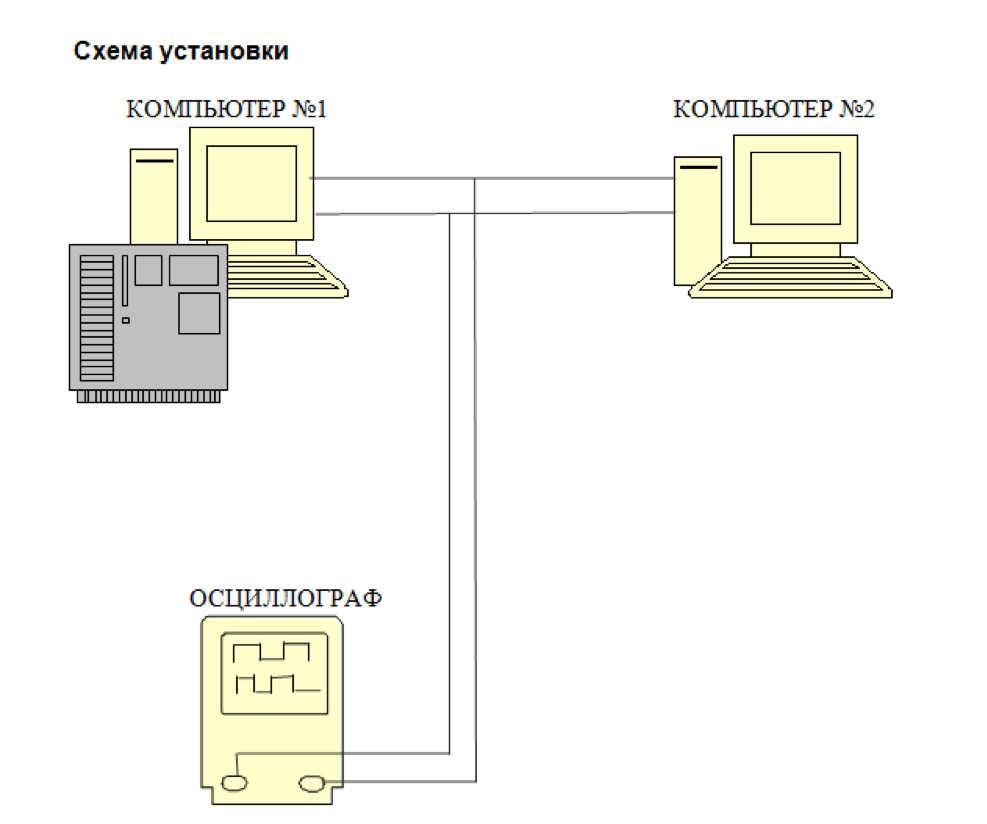
\includegraphics[width=\textwidth]{img/scheme.png}
	\caption{схема лабораторной установки}
\end{figure}



\chapter{Ход работы}

В первом пункте работы исследуется зависимость коэффициента передачи материала от частоты сигнала. Приёмник устанавливается в непосредственной близости к источнику, а замет на удалении от него. В обоих случаях фиксируются уровни принимаемого сигнала в зависимости от его частоты. По результатам измерения заполнена таблица \ref{tbl:1}



\begin{table}
	\centering
	\caption{}
	\label{tbl:1}
	\begin{tabular}{|c|c|c|c|}
		\hline
		$f$, Гц & $U_{c1}$, В & $U_{c2}$, В & $Q$ \\ \hline
		250 & 0.04 & 0.030 & 1.43\\ \hline
		500 & 0.03 & 0.020 & 1.5 \\ \hline
		1000 & 0.025 & 0.015 & 1.6 \\ \hline
		2000 & 0.020 & 0.014 & 1.35 \\ \hline
		4000 & 0.010 & 0.05 & 2 \\ \hline 
	\end{tabular}
\end{table}

\begin{tikzpicture}
\begin{axis}[
title={Зависимость коэффициента передачи от частоты.},
xlabel={Частота, Гц},
ylabel={Q},
xmin=200, xmax=4200,
ymin=0, ymax=3,
legend pos=north west,
ymajorgrids=true,
grid style=dashed,
]

\addplot[
color=blue,
mark=square,
smooth
]
coordinates {
(250, 1.43)(500, 1.5)(1000, 1.6)(2000, 1.35)(4000, 2)
};
\end{axis}
\end{tikzpicture}

Во втором пункте работы исследуется активная акустическая
защита с использованием генератора шума. Источник и приёмник
устанавливаются на удалении друг от друга, а между ними ставится
вибропреобразователь, подключенный к источнику шума.

Положение преобразователя изменяется, и для каждого положения
фиксируется уровень суммарного принимаемого сигнала и уровень
шума. На основании измерений вычисляется соотношение сигнал-шум. Измерения приведены в таблице \ref{tbl:2}.

\begin{table}[H]
	\centering
	\caption{}
	\label{tbl:2}
	\begin{tabular}{|c|c|c|c|}
		\hline
		Положение & $U_\text{с+щ}$, В & $U_\text{ш}$, В & $ \Delta i$ \\ \hline
		1 & 0.045 & 0.06 & 0.75 \\ \hline
		2 & 0.045 & 0.06 & 0.75 \\ \hline
		3 & 0.050 & 0.06 & 0.8 \\ \hline
		4 & 0.080 & 0.06 & 1.3 \\ \hline
		5 & 0.080 & 0.07 & 1.1 \\ \hline
	\end{tabular}
\end{table}

\begin{tikzpicture}
\begin{axis}[
title={ Зависимость соотношения сигнал-шум от положения
	вибропреобразователя.},
xlabel={Положение},
ylabel={$\Delta i$},
xmin=0, xmax=6,
ymin=0, ymax=2,
legend pos=north west,
ymajorgrids=true,
grid style=dashed,
]

\addplot[
color=blue,
mark=square,
smooth
]
coordinates {
 (1, 0.75) (2, 0.75) (3, 0.8) (4, 1.3) (5, 1.1)
};
\end{axis}
\end{tikzpicture}
